\hypertarget{a00826}{}\section{Plug-\/in type conversion}
\label{a00826}\index{Plug-\/in type conversion@{Plug-\/in type conversion}}
Specification for valid conversions between plug-\/in types. 

\hypertarget{a00826_advancedTopics_relatedTypes_about}{}\subsection{About this specification}\label{a00826_advancedTopics_relatedTypes_about}
The specification on this page defines the valid A\+AX plug-\/in type conversions. An A\+AX host may use this specification to perform automatic type conversions. For example\+: 
\begin{DoxyItemize}
\item When a session that was saved with a D\+SP plug-\/in Type is opened on a Native system the saved D\+SP Type should be converted to its Native counterpart.  
\item When a session saved with the free version of a plug-\/in is opened on a system that has the full version installed then the saved free Type may be converted to the full version.  
\end{DoxyItemize}\hypertarget{a00826_advancedTopics_relatedTypes_terminology}{}\subsection{Terminology}\label{a00826_advancedTopics_relatedTypes_terminology}
In this specification the term \char`\"{}\+Type\char`\"{} refers to a specific configuration of an A\+AX plug-\/in.

Each Type is uniquely identified by a combination of five values\+: 
\begin{DoxyItemize}
\item Manufacturer ID  
\item Product ID  
\item Plug-\/\+In ID  
\item Sample rate bit mask  
\item Architecture  
\end{DoxyItemize}

Each Type is defined by a particular call to \mbox{\hyperlink{a01781_a1c069508cf54a523905c8160ebf628ad}{A\+A\+X\+\_\+\+I\+Component\+Descriptor\+::\+Add\+Process\+Proc\+\_\+\+Native}} or \mbox{\hyperlink{a01781_a38f7fb30a378a17ce9635f5c36100a3b}{A\+A\+X\+\_\+\+I\+Component\+Descriptor\+::\+Add\+Process\+Proc\+\_\+\+TI}} in the plug-\/in\textquotesingle{}s description method.

The Plug-\/\+In ID is defined as one of \mbox{\hyperlink{a00662_a13e384f22825afd3db6d68395b79ce0da89ca3dd6e96895cda14976c1b1ceb826}{A\+A\+X\+\_\+e\+Property\+\_\+\+Plug\+In\+I\+D\+\_\+\+Native}} or \mbox{\hyperlink{a00662_a13e384f22825afd3db6d68395b79ce0da75f174df4efbeca86eaada126c1d9214}{A\+A\+X\+\_\+e\+Property\+\_\+\+Plug\+In\+I\+D\+\_\+\+TI}}.

In this specification, the format for describing an ID is\+:

\mbox{[} ID triad + sample rate + architecture \mbox{]}

Where the ID triad may be expanded to \mbox{[} \mbox{[}Manufacturer ID\mbox{]} \mbox{[}Product ID\mbox{]} \mbox{[}Plug-\/\+In ID\mbox{]} \mbox{]}


\begin{DoxyItemize}
\item Explicit values are given in plain face  
\item Arbitrary constant values are given in {\itshape bold face}  
\item Wildcard values are given in {\itshape italics}  
\end{DoxyItemize}

For example\+: 
\begin{DoxyItemize}
\item \mbox{[} {\itshape ID triad} + {\itshape any sample rate} + Native \mbox{]} 
\begin{DoxyItemize}
\item Defines all Type identifiers with the same ID triad and the Native architecture, regardless of sample rate.  
\end{DoxyItemize}
\item \mbox{[} \mbox{[} \mbox{[}{\itshape Manufacturer ID}\mbox{]} \mbox{[}{\itshape Product ID}\mbox{]} \mbox{[}{\itshape any ID}\mbox{]} \mbox{]} + {\itshape sample rate} + Native \mbox{]} 
\begin{DoxyItemize}
\item Defines all Type identifiers with the same Manufacturer and Product I\+Ds, the same sample rate, and the Native architecture, but with any plug-\/in ID.  
\end{DoxyItemize}
\end{DoxyItemize}\hypertarget{a00826_advancedTopics_relatedTypes_scope}{}\subsection{Scope of this specification}\label{a00826_advancedTopics_relatedTypes_scope}
For the purposes of this specification we are not concerned with Audio\+Suite Types. Currently these Types are never type-\/converted.

In theory, an A\+AX host may apply a \char`\"{}partial\char`\"{} type conversion by swapping between different Process\+Procs without destroying and re-\/building any of the plug-\/in\textquotesingle{}s objects (data model, G\+UI). For the purposes of this specification we are not concerned about whether a given conversion is \char`\"{}partial\char`\"{} or \char`\"{}total\char`\"{}; all conversions are treated the same.

Plug-\/in conversions are also required between Types of different stem formats. In fact, the supported stem format is an integral part of a Type\textquotesingle{}s unique identifier. This specification ignores the question of stem formats entirely; we assume that each Type supports all necessary stem formats for legal conversion with other Types.

In general, type swapping rules for deprecated types and related types are equivalent. See \mbox{\hyperlink{a00826_advancedTopics_relatedTypes_deprecation}{Type deprecation}} for more information about the differences between related and deprecated types.\hypertarget{a00826_advancedTopics_relatedTypes_constraints}{}\subsection{Topological constraints}\label{a00826_advancedTopics_relatedTypes_constraints}

\begin{DoxyItemize}
\item All Types included in a single \mbox{\hyperlink{a01777}{A\+A\+X\+\_\+\+I\+Collection}} must have the same Manufacturer ID  
\item All Types included in a single \mbox{\hyperlink{a01813}{A\+A\+X\+\_\+\+I\+Effect\+Descriptor}} must have the same Manufacturer ID and Product ID  
\item The Sample rate bit masks for two Types that share all other identifiers must be non-\/overlapping. I.\+e. {\ttfamily 0x0 == sr\+\_\+mask1 \& sr\+\_\+mask2}  
\item Two Types may not be registered that differ only in their Architecture  
\item Type relationships may only be defined between mutually exclusive Types. Types are mutually exclusive if\+: 
\begin{DoxyItemize}
\item Their sample rate support is non-\/overlapping  
\item The \char`\"{}before\char`\"{} Type\textquotesingle{}s ID triad is not associated with any Type in the plug-\/in  
\end{DoxyItemize}
\end{DoxyItemize}\hypertarget{a00826_advancedTopics_relatedTypes_implicitconversions}{}\subsection{Implicit conversions}\label{a00826_advancedTopics_relatedTypes_implicitconversions}
The A\+AX host should automatically convert between Types within the following I\+Ds\+: 
\begin{DoxyItemize}
\item \mbox{[} {\itshape ID triad} + {\itshape any sample rate} + {\itshape Architecture} \mbox{]}  
\item \mbox{[} \mbox{[} \mbox{[}{\itshape Manufacturer ID}\mbox{]} \mbox{[}{\itshape Product ID}\mbox{]} \mbox{[}{\itshape any ID}\mbox{]} \mbox{]} + {\itshape sample rate} + {\itshape any architecture} \mbox{]}  
\end{DoxyItemize}

These conversions occur only if both Types are included in the plug-\/in when the conversion is made. Consider the following scenario\+: 
\begin{DoxyEnumerate}
\item A session is saved including an plug-\/in instance with the following Type identifier\+: \mbox{[} My ID triad + 48 k\+Hz + TI \mbox{]}  
\item The plug-\/in is updated to a version that does not include this Type identifier, but that does include \mbox{[} My ID triad + 48 k\+Hz + Native \mbox{]}  
\item The session is opened on a Native system  
\end{DoxyEnumerate}

In this scenario, if the plug-\/in had not been updated then an automatic conversion would occur. However, since the plug-\/in no longer includes the saved Type identifier, no automatic conversion occurs.

A plug-\/in can work around this situation by including the \char`\"{}old\char`\"{} Type identifier as a Related (or Deprecated) Type (see \mbox{\hyperlink{a00826_advancedTopics_relatedTypes_explicitconversions}{Explicit conversions}}.)

When a plug-\/in instance is saved after making an implicit conversion, plug-\/ins may be saved with the session using their new Type identifier. This is not required. For example, Pro Tools will prefer to save plug-\/in instances that were converted from D\+SP types as D\+SP, even if they were converted to corresponding Native types when the session was loaded onto and saved from a native Pro Tools system.\hypertarget{a00826_advancedTopics_relatedTypes_explicitconversions}{}\subsection{Explicit conversions}\label{a00826_advancedTopics_relatedTypes_explicitconversions}
A\+AX includes properties that allow a plug-\/in to define explicit relationships between different Types. These properties only operate on ID triads. Each property can be associated with an array of ID triads to define a one-\/to-\/one or a many-\/to-\/one association between the given ID triads and the specific Type to which the property is attached. 
\begin{DoxyItemize}
\item \mbox{\hyperlink{a00662_a13e384f22825afd3db6d68395b79ce0da9dc35184d705e963f14f85df4d71193d}{A\+A\+X\+\_\+e\+Property\+\_\+\+Related\+\_\+\+D\+S\+P\+\_\+\+Plugin\+\_\+\+List}} / \mbox{\hyperlink{a00662_a13e384f22825afd3db6d68395b79ce0dab102bc794f2770c14b1f0fe2dde6766a}{A\+A\+X\+\_\+e\+Property\+\_\+\+Deprecated\+\_\+\+D\+S\+P\+\_\+\+Plugin\+\_\+\+List}} 
\begin{DoxyItemize}
\item All of the given ID triads specify TI Types  
\end{DoxyItemize}
\item \mbox{\hyperlink{a00662_a13e384f22825afd3db6d68395b79ce0dae47f50370ae2f6bf29b8cacc6a41d924}{A\+A\+X\+\_\+e\+Property\+\_\+\+Related\+\_\+\+Native\+\_\+\+Plugin\+\_\+\+List}} / \mbox{\hyperlink{a00662_a13e384f22825afd3db6d68395b79ce0da3f1e690c987d601001a7cc1da8247399}{A\+A\+X\+\_\+e\+Property\+\_\+\+Deprecated\+\_\+\+Native\+\_\+\+Plugin\+\_\+\+List}} 
\begin{DoxyItemize}
\item All of the given ID triads specify Native Types  
\end{DoxyItemize}
\end{DoxyItemize}

The A\+AX host should convert between related Types within the following constraints\+: 
\begin{DoxyItemize}
\item \mbox{[} \mbox{[} \mbox{[}Manufacturer ID\mbox{]} \mbox{[}Related Product ID\mbox{]} \mbox{[}Related TI Plug-\/\+In ID\mbox{]} \mbox{]} + {\itshape sample rate} + TI \mbox{]} 
\begin{DoxyItemize}
\item -\/$>$ \mbox{[} \mbox{[} \mbox{[}Manufacturer ID\mbox{]} \mbox{[}New Product ID $\vert$ Related Product ID\mbox{]} \mbox{[}New Plug-\/\+In ID\mbox{]} \mbox{]} + {\itshape sample rate} + {\itshape any architecture} \mbox{]}  
\end{DoxyItemize}
\item \mbox{[} \mbox{[} \mbox{[}Manufacturer ID\mbox{]} \mbox{[}Related Product ID\mbox{]} \mbox{[}Related Native Plug-\/\+In ID\mbox{]} \mbox{]} + {\itshape sample rate} + Native \mbox{]} 
\begin{DoxyItemize}
\item -\/$>$ \mbox{[} \mbox{[} \mbox{[}Manufacturer ID\mbox{]} \mbox{[}New Product ID $\vert$ Related Product ID\mbox{]} \mbox{[}New Plug-\/\+In ID\mbox{]} \mbox{]} + {\itshape sample rate} + {\itshape any architecture} \mbox{]}  
\end{DoxyItemize}
\end{DoxyItemize}

These conversions will occur regardless of whether the related ID triad is used for any of the Types in the plug-\/in.

When a plug-\/in instance is saved after making an explicit conversion, all plug-\/ins are saved with the session using their new Type identifier.

\begin{DoxyRefDesc}{Host Compatibility Notes}
\item[\mbox{\hyperlink{a00786__compatibility_notes000009}{Host Compatibility Notes}}]Pro Tools versions prior to Pro Tools 12.\+3 do not allow explicit type conversion between types with different product ID values. Beginning in Pro Tools 12.\+3 both the product ID and the plug-\/in ID may differ between explicitly related types.\end{DoxyRefDesc}
\hypertarget{a00826_advancedTopics_relatedTypes_deprecation}{}\subsection{Type deprecation}\label{a00826_advancedTopics_relatedTypes_deprecation}
There are two varieties of explicit plug-\/in type association\+: related types and deprecated types.

Properties that create a related type association\+: 
\begin{DoxyItemize}
\item \mbox{\hyperlink{a00662_a13e384f22825afd3db6d68395b79ce0dae47f50370ae2f6bf29b8cacc6a41d924}{A\+A\+X\+\_\+e\+Property\+\_\+\+Related\+\_\+\+Native\+\_\+\+Plugin\+\_\+\+List}} 
\item \mbox{\hyperlink{a00662_a13e384f22825afd3db6d68395b79ce0da9dc35184d705e963f14f85df4d71193d}{A\+A\+X\+\_\+e\+Property\+\_\+\+Related\+\_\+\+D\+S\+P\+\_\+\+Plugin\+\_\+\+List}} 
\end{DoxyItemize}

Properties that create a deprecated type association\+: 
\begin{DoxyItemize}
\item \mbox{\hyperlink{a00662_a13e384f22825afd3db6d68395b79ce0da3f1e690c987d601001a7cc1da8247399}{A\+A\+X\+\_\+e\+Property\+\_\+\+Deprecated\+\_\+\+Native\+\_\+\+Plugin\+\_\+\+List}} 
\item \mbox{\hyperlink{a00662_a13e384f22825afd3db6d68395b79ce0dab102bc794f2770c14b1f0fe2dde6766a}{A\+A\+X\+\_\+e\+Property\+\_\+\+Deprecated\+\_\+\+D\+S\+P\+\_\+\+Plugin\+\_\+\+List}} 
\item \mbox{\hyperlink{a00662_a13e384f22825afd3db6d68395b79ce0dadb254df9b6114516beed7a04675a22a3}{A\+A\+X\+\_\+e\+Property\+\_\+\+Plug\+In\+I\+D\+\_\+\+Deprecated}} 
\end{DoxyItemize}

With a few exceptions, these two types of explicit association are treated identically. These are the ways in which deprecated plug-\/in type association differs from related plug-\/in type association\+: 
\begin{DoxyItemize}
\item If plug-\/in types A and B are both installed, and if type A deprecates type B, then type B will be excluded from all insert lists in Pro Tools and will be made invisible to the user. 
\item If plug-\/in types A and B are both installed, and if type A deprecates type B, then instances of type B will be swapped to type A when a session containing saved instances of type B is opened. 
\item Upon the next session save following a swap due to a deprecated type association, the plug-\/in instance will be saved into the session using the ID of the new plug-\/in type. Therefore deprecated type swaps do not round-\/trip when moving between multiple systems if some of the systems have the deprecated types, but not the deprecating types, installed. 
\end{DoxyItemize}

Type deprecation should only be used when a new version of an effect completely replaces an old version of the effect. For all other situations, type relationship should be used.

\begin{DoxyRefDesc}{Host Compatibility Notes}
\item[\mbox{\hyperlink{a00786__compatibility_notes000010}{Host Compatibility Notes}}]\end{DoxyRefDesc}
\begin{DoxyItemize}
\item Pro Tools versions before Pro Tools 12.\+3 treat deprecated and related type associations identically and do not support type deprecation features \item Media Composer does not support type deprecation features \item V\+E\+N\+UE does not support type deprecation features \end{DoxyItemize}
Collaboration diagram for Plug-\/in type conversion\+:
\nopagebreak
\begin{figure}[H]
\begin{center}
\leavevmode
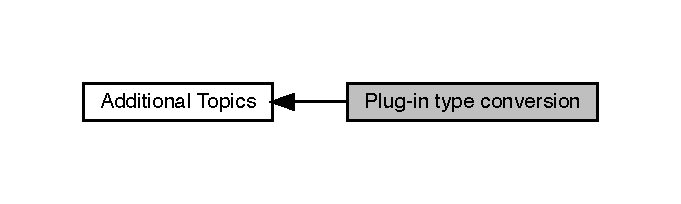
\includegraphics[width=327pt]{a00826}
\end{center}
\end{figure}
